\section*{05-13 - Supernovae}
Una volta scoperto il neutrone nel 1932 ci sono voluti pochi anni dalla prima predizione dell'esistenza delle stelle di neutroni. Nel 1933 W. Baade e F. Zwicky suggeriscono l'esistenza di oggetti così compatti da essere fatti soltanto da neutroni. In quel periodo studiavano le supernovae, alcuni tra i processi più energetici del cosmo e per giustificare l'energia emessa da questi oggetti suggerirono che questa energia provenisse dal collasso gravitazionale del core di una stella massiccia che passa dalle dimensioni tipiche del core di una stella massiccia a quelle di una stella di neutroni. Proprio nell'articolo pubblicato suggeriscono che le densità che si vengono a trovare siano confrontabili con quelle dei nuclei atomici. Sempre nel 1934 Chandrasekhar insieme a von Neumann riscrivono le equazioni dell'equilibrio idrostatico tenendo conto della relatività generale proprio per descrivere la fisica di oggetti così compatti. Non pubblicheranno questo risultato che verrà poi reso pubblico nel 1939 da Tolman - Oppenheimer e Volkov indipendentemente.\\
Per i decenni successivi ci si dimentica delle stelle di neutroni, che non erano altro che speculazioni teoriche. La prima evidenza sperimentale risale al 1967/68 quando viene scoperta la prima pulsar.\\
L'11 Novembre 1572 nella costellazione di Cassiopea è comparsa una nuova stella, talmente brillante da avere luminosità apparente simile a quella di Giove. Uno dei più grandi studiosi di questo evento fu Tycho Brahe. Egli provò a misurarne la parallasse, che però risultò inferiore alla risoluzione dello strumento, il che implicò che l'oggetto dovesse essere oltre la sfera della Luna, cosa che determinò la crisi del modello per il quale oltre questa sfera tutto fosse immutabile. Oggi sappiamo che quella non era una stella ma una supernova, la supernova di Tycho (SN 1572). Oggi vediamo i resti dell'esplosione, e vediamo gli strati che si stanno espandendo a migliaia di km al secondo. Sappiamo che corrisponde ad un particolare tipo di supernova, le SN Ia e corrisponde all'esplosione di una nana bianca che ha superato la $M_{Ch}$.
\subsection*{Classificazione SN}
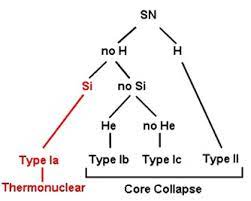
\includegraphics{images/snclass.jpg}
La prima classificazione si bassa sullo studio dello spettro. La prima biforcazione compara la  presenza di $\ce{H}$. Se è presente sono di tipo II altrimenti di tipo I. Se tra le I è presente il Si, allora si parla di tipo Ia, altrimenti si passa a valutare la presenza di He: se è presente sono le Ib, altrimenti Ic. Le Ia sono chiamate termonucleari, mentre le altre sono chiamate Core Collapse. Ci rendiamo quindi conto che le II, Ib e Ic hanno come progenitore una stella massiccia ($M.9.5\sunmass$). La differenza tra questi tre casi è nella parte più esterna. Le tipo II hanno avuto una perdita di massa che non ha eroso lo strato più esterno ricco di H. Se la perdita di massa è abbastanza efficiente da erodere tutto l`inviluppo esterno prima che la stella esploda non abbiamo più idrogeno nel momento dell'esplosione. Quindi la differenza sta nell'efficienza della perdita di massa prima che la stella esploda.
\subsubsection*{Instabilità}
Abbiamo la struttura del core a cipolla, con un core di ferro circondato dalla shell in silicio e via dicendo. Sappiamo che il core è il risultato della combustione del silicio da cui viene prodotto il ferro. Perché a quel punto diventa instabile? Sappiamo che la shell di silicio è attiva, quindi bruciando produce ferro che fa aumentare la massa del core. Quindi il core è elettronicamente degenere, inerte e aumenta in massa. È come se avessimo una nana bianca dentro la stella massiccia. Ciò implica che la sua massa non può aumentare a piacere poiché esiste il limite di Chandrasekhar. Facendo il calcolo, sappiamo che $\mu_e\approx2.15$ che sostituito nella formula della massa limite otteniamo $M_{Ch}\approx 1.25\sunmass$. Quindi quando il core raggiunge questa massa si ha un'instabilità. Si attiveranno i processi di cattura elettronica
\begin{equation*}
    (A,Z)+e^- \to (A, Z-1)+\nu_e
\end{equation*}
Sappiamo che la pressione è dominata dalla pressione degli elettroni degeneri. Questo processo, sottraendo elettroni, sottrae pressione. Ci aspettiamo quindi che l'equilibrio idrostatico non sia soddisfatto ed inizia il collasso del core. Durante il collasso aumenta la densità, quindi l'energia degli elettroni degeneri, il che amplifica il processo di cattura elettronica. Nel collasso inoltre il core si sta scaldando e una volta raggiunte $T\approx (6\div7)\times10^9$ i fotoni fotodisintegrano i nuclei di ferro producendo elio:
\begin{equation*}
    \ce{{}^{56}Fe +{\gamma}  -> 13{}^{4}He +4n}
\end{equation*}
Per ogni nucleo di ferro, questo processo sottrae $100$ MeV. Stiamo facendo il percorso opposto a quello di una stella, tornando indietro nel diagramma di energia di legame vs numero di massa, sottraendo energia alla stella, fino a quando non si raggiunge la temeperatura che fotodisintegra i nuclei di elio:
\begin{equation*}
    \ce{^{4}He + {\gamma} -> 2p + 2n}
\end{equation*}
Che sottrae $27$ MeV per ogni nucleo di elio. Così finché non si passa all'idrogeno. I neutroni prodotti in questa maniera non decadono, le densità sono tali da far sì che ad un elettrone convenga legarsi ad un protone piuttosto che stare libero. Quello che si ottiene alla fine è un oggetto costituito principalmente da neutroni. I tempi scala con cui abbiamo a che fare sono tempi scala di caduta libera del core di ferro, $\tau_{\text{ff}}\approx 1/\sqrt{G\Bar{\rho}}\sim 1\um{s}$.\\
L'energia che si libera durante il collasso si può scrivere come ($R_{\ce{Fe}}\sim 10^4\um{km}$, $R_{\text{NS}}\sim 20\um{km}$, $M_{\ce{Fe}}\sim1.25\sunmass$):
\begin{equation*}
    \Delta E_{\text{grav}}\approx -GM_{\ce{Fe}}^2\left( \frac{1}{R_{\ce{Fe}}}-\frac{1}{R_{\text{NS}}}\right)\approx 2\times 10^{53}\um{erg}.
\end{equation*}
Nel giro di un secondo, nel corso del collasso del core, viene liberata un'energia superiore a quella liberata da stelle come il sole in tutta la loro vita. La maggior parte dell'energia viene espulsa in neutrini.\\
Cosa succede per le supernovae di tipo Ia? Il progenitore di queste non è una stella massiccia ma una nana bianca che ha raggiunto la massa limite di Chandrasekhar. Osservando Algol (beta persei) ci accorgiamo che è un sistema binario ad eclisse. Sappiamo che in questo tipo di sistema riusciamo a stimare la massa e diamo il nome di Algol A a quella più massiccia, e Algol B a quella meno massiccia. (pag 24 supernovae) Scopriamo, attraverso il diagramma HR che Algol B è subgigante, Algol A è in sequanza principale. Ma noi sappiamo che il tempo scala con cui si evolve una stella, diminuisce al cresceere della massa di una stella. Allora perché Algol appare paradossale? La soluzione si ha rendendosi conto del fatto che il sistema è un sistema binario. Nel sistema di riferimento corotante possiamo scrivere il potenziale efficace. Guardando le superfici equipotenziali otteniamo superfici del tipo pag. 28. I lobi che vediamo prendono il nome di Lobi di Roche. Finché la superficie stella sta all'interno del proprio lobo di Roche, essa si evolve come se fosse singola. Se (o quando) la stella riempie il proprio lobo di roche, la materia arriva al punto $L_1$ e parte della stessa riesce a piovere sull'altra stella: c'è il così detto trasferimento di massa. Pag. 29 per le definizioni. Oggi Algol B ha una massa inferiore di Algol A a causa del trasferimento di massa. Questo ci permette di capire come si sono formate le supernovae di tipo Ia: abbiamo bisogno che una nana bianca raggiunga la massa limite di Chandrasekhar. Siccome si pensa che l'evoluzione di massa singola non produca un numero sufficiente di questi oggetti, si deve ricorrere ai sistemi binari. Solitamente si parla di due stistemi:
\begin{itemize}
    \item Singolo degenere: una nana bianca ed un'altra no. La stella che non è nana bianca diventa gigante rossa, riempie il lobo di roche e trasferisce materia alla nana bianca. Si parla di supernovae di tipo termonucleare perché la nana bianca si sta scaldando, fino a quando non innesca il carbonio e, essendo l'ambiente degenere, si ha un effetto a catena che aumenta temperatura e di conseguenza i rate nucleari che rilasciano abbastanza energia da distruggere la struttura. Questo effetto a catena che distrugge la stella prende il nome di \textit{runaway nucleare} Si pensa che non lasci alcun oggetto compatto, che dissolvano la struttura.
    \item Doppio degenere: sistema binario con due nane bianche. Queste spiraeggiano fino ad un merging. Se la somma delle masse supera $M_{\text{Ch}}$ si ha un'esplosione.
\end{itemize}
Nel runaway nucleare si produce \ce{{}^{56}Ni} invece che \ce{{}^{56}Fe} perché l'esplosione avviene in tempi scala brevi. Inoltre la composizione chimica della materia iniziale è costituita da nuclei atomici che hanno lo stesso numero di protoni e neutroni ed il tempo scala è talmente breve da non permettere un numero significativo di decadimenti beta. Quindi l'equilibrio nucleare statistico tende a produrre nuclei che abbiano lo stesso numero di protoni e di neutroni, cioé il \ce{{}^{56}Ni}. D'altra parte il \ce{{}^{56}Ni} è instabile:
\begin{equation*}
    \ce{{}^{56}Ni -> {}^{56}Co + e+ + \nu_e}, \quad \tau_{1/2}\sim 6.1 \um{giorni}
\end{equation*}
Il cobalto a sua volta è instabile e si ha 
\begin{equation*}
    \ce{{}^{56}Co -> {}^{56}Fe + e+ + \nu_e}, \quad \tau_{1/2}\sim 77.7\um{giorni}
\end{equation*}
Ci aspettiamo che la materia sia eiettata ad altissima velocità ($\gtrsim 10^4\um{km/s}$) e che sia composta principalmente da $\ce{^{56}Ni}$ e che questo decada producendo il cobalto, poi ferro e dopo parecchio tempo che decada anche quest'ultimo. Ci aspettiamo che questo decadimento produca una certa luminosità. So che quando ho un decadimento radioattivo il numero di particelle cambia come
\[ \frac{dN}{dt}=-\lambda N\Rightarrow N(t)=N_0e^{-\lambda t}\]
Conoscendo $\tau_{1/2}$, sappiamo
\[
    \frac{1}{2}N_0=N_0e^{-\lambda \tau_{1/2}} \Rightarrow \lambda = \frac{\ln 2}{\tau_{1/2}}
\]
E ci aspettiamo per la luminosità
\[
    L \propto N \propto e^{-\lambda t} \Rightarrow \log L \propto -\lambda t + \text{cost.}
\]
Quindi ci aspettiamo un andamento fatto come a pag. 35 supernovae: nella prima parte il decadimento del nichel nella seconda quella del cobalto.
\subsubsection*{Esplosione di supernova}
Il fenomeno è transitorio.  Si osseva la curva di luce che da la magnitudine in funzione del tempo. Quello che si osserva è un andamento in cui la luminosità inizialmente aumenta, raggiunge un picco e poi decresce (pag. 21 supernovae). La curva sembra una spezzata.
\subsection*{Stelle di neutroni - caratteristiche}
Quando sono state scoperte le pulsar alla fine degli anni '60, esse emettevano un segnale periodico con $1 \um{ms} < P < 10 \um{s}$. Da quasi subito è stato previsto che il meccanismo che garantisce regolarità (numero di cifre significative confrontabile a quelle di un orologio atomico) al processo era la rotazione. Si associa quindi il periodo del segnale a quello di rotazione, ed un periodo così piccolo implica grandi densità. Noi vogliamo che l'oggetto non venga disgregato dalla rotazione e quindi che
\[
\Omega^2R < G\frac{M}{R^2}\quad \Rightarrow \quad \Omega^2 < G\frac{M}{R^3}\quad \Rightarrow \quad \Omega < \sqrt{\frac{4}{3}\pi G \Bar{\rho}}
\]
\[
    \Rightarrow \quad \Bar{\rho} > \frac{3}{4\pi} \frac{\Omega^2}{G} = \frac{3\pi}{G}\frac{1}{P^2},\quad P = \frac{2\pi}{\Omega}
\]
\[
    P \sim \um{ms}\quad \Rightarrow \quad \Bar{\rho} \sim 10^{14} \um{g/cm}^3
\]
Fu questo risultato a far supporre che in realtà fossero stelle di neutroni. Tipicamente le stelle di neutroni hanno $M\sim1.4\sunmass$, $R\sim10\um{km}$ e quindi $\Bar{\rho} \sim 7\times 10^{14}\um{g/cm}^3$. La densità media nucleare è $\rho_0 = 2.8\times10^{14}\um{g/cm}^3$ (nuclear normal density) e vediamo che $\Bar{\rho}=(2\div 3)\rho_0$ e la densità centrale di questi oggetti raggiunge valori di $\rho_c\sim (10\div 20)\rho_0$. Chiaramente, gli effetti della relatività generale non possono più essere trascurati essendo il raggio della NS paragonabile al raggio di Schwarzschild.\\
Cosa succede se facciamo precipitare un oggetto di massa $m$ dall'infinito su un oggetto di massa $M$ e raggio $R$? Avremo una variazione di energia potenziale del tipo
\[ 
G\frac{Mm}{R} = \frac{GM}{c^2R}mc^2
\]
Per le stelle di neutroni abbiamo che
\[
    \frac{GM}{c^2R}\sim (0.1\div0.15)
\]
Questo implica che la quantità di energia che viene liberata in questo processo rispetto a $mc^2$ è dell'ordine del $(10\div15)\%$. Questo è un numero enorme rispetto alla frazione di energia a riposo liberata nelle reazioni nucleari. Abbiamo visto che nel caso della combustione di H (4 protoni diventano un nucleo di elio) lo 0.7\% dell'energia a riposo viene liberata e che in generale la massima energia che può essere liberata con reazioni termonucleari (convertendo idrogeno in ferro) sarebbe dello 0.85\%. La caduta di materia su oggetti estremamente compatti è il fenomeno più energetico dell'universo.

\subsection*{SN Ia come candele standard}
Sappiamo che una delle misure più difficili in astronomia è quella delle distanze. Le misure dirette sono possibili solo per distanze relativamente piccole (con Gaia non usciamo dalla Via Lattea). Per sopperire a ciò usiamo metodi indiretti. Questi si bassano principalmente sulle candele standard: se abbiamo un oggetto del quale conosciamo a priori la luminosità intrinseca, allora se osserviamo l'oggetto e ne misuriamo la luminosità apparente, otteniamo la distanza dall'oggetto. Abbiamo bisogno di candele standard per ogni distanza. Si utilizzeranno candele con alcune classi di luminosità per certe distanze, e luminosità maggiori per distanze maggiori. C'è bisogno che queste candele siano uniformate per creare una scala. Per distanze cosmologiche abbiamo bisogno di oggetti estremamente luminosi, le supernovae Ia. Nel 1993 si è visto che era possibile utilizzare le Ia come candele campione ed essendo molto luminose si riescono a valutare distanze dell'ordine di Gpc. A pag. 63 supernovae vediamo il confronto tra la luminosità di una supernova (gialla) e quella di una galassia (rossa) poste alla stessa distanza. L'esplosione di un singolo oggetto produce, per breve tempo, una quantità di luce confrontabile a quella ottenuta sommando quella prodotta da una galassia di stelle.